\documentclass{article}
%\usepackage[T1]{fontenc}
\usepackage{amsmath}
\usepackage{fancyhdr}
\usepackage{amssymb}
\usepackage{amsthm}
\usepackage{graphicx}
\usepackage{varioref}
\usepackage{verbatim} 
\usepackage{multicol}
\usepackage{enumerate}

\usepackage{mathtools}
%\usepackage[normalem]{ulem}

\usepackage{caption}
\usepackage{subcaption}
%\usepackage[T1]{fontenc}
\usepackage[margin=1in]{geometry}
\usepackage{qcircuit}

%\usepackage{mathrsfs}

\usepackage{url}\urlstyle{same}
\usepackage{xspace}
\usepackage{thm-restate}

% Nicer font
%\usepackage{mathpazo}

% Microtype
\usepackage{microtype}

% TikZ
\usepackage{tikz}
\usetikzlibrary{decorations.pathreplacing}
\usetikzlibrary{calc}

% Support eps figures
\usepackage{epstopdf}

% Hypertext package
\usepackage[colorlinks = true]{hyperref}
% Title and authors
%\hypersetup{
%  pdftitle = {},
%  pdfauthor = {}
%}
% Color definitions
\usepackage{xcolor}
\definecolor{darkred}  {rgb}{0.5,0,0}
\definecolor{darkblue} {rgb}{0,0,0.5}
\definecolor{darkgreen}{rgb}{0,0.5,0}
% Color links
\hypersetup{
  urlcolor   = blue,         % color of external links
  linkcolor  = darkblue,     % color of internal links
  citecolor  = darkgreen,    % color of links to bibliography
  filecolor  = darkred       % color of file links
}

% Clever references
\usepackage{cleveref}%[nameinlink]
\crefname{lemma}{Lemma}{Lemmas}
\crefname{proposition}{Proposition}{Propositions}
\crefname{definition}{Definition}{Definitions}
\crefname{theorem}{Theorem}{Theorems}
\crefname{conjecture}{Conjecture}{Conjectures}
\crefname{corollary}{Corollary}{Corollaries}
\crefname{section}{Section}{Sections}
\crefname{appendix}{Appendix}{Appendices}
\crefname{figure}{Fig.}{Figs.}
\crefname{equation}{Eq.}{Eqs.}
\crefname{table}{Table}{Tables}
\crefname{claim}{Claim}{Claims}


%%%%%%%%%%%%%%%%%%%%%%%%%
%  N E W T H E O R E M  %
%%%%%%%%%%%%%%%%%%%%%%%%%

\newtheorem{theorem}{Theorem}
\newtheorem{lemma}[theorem]{Lemma}
\newtheorem{proposition}[theorem]{Proposition}
\newtheorem{definition}[theorem]{Definition}
\newtheorem{corollary}[theorem]{Corollary}
\newtheorem{conjecture}[theorem]{Conjecture}
\newtheorem*{conjecture*}{Conjecture}
\newtheorem*{problem}{Problem}
\newtheorem{claim}[theorem]{Claim}
\theoremstyle{definition}
\newtheorem*{remark}{Remark}
\newtheorem*{example}{Example}


%%%%%%%%%%%%%%%%%%%
%  Comments  %
%%%%%%%%%%%%%%%%%%%
\newcommand{\todo}[1]{{\color{red}{[{\bf TODO:} #1]}}}
\newcommand{\tocite}[1]{{\color{blue}{[{\bf CITE:}#1]}}}
\newcommand{\tocheck}[1]{{\color{red}{[{\bf TO CHECK:}#1]}}}

%%%%%%%%%%%%%%%%%%%
%  Author Affiliations  %
%%%%%%%%%%%%%%%%%%%
%\usepackage{authblk}
%\renewcommand\Authfont{\scshape}
%\renewcommand\Affilfont{\itshape\small}


%%%%%%%%%%%%%%%%%%%
%  New Commands  %
%%%%%%%%%%%%%%%%%%%


\newcommand{\ee}{\mathcal{E}}
\newcommand{\ii}{\mathbb{I}}
\newcommand{\rl}{\rangle\langle}
\newcommand{\mg}{\mathcal{G}}
\newcommand{\hn}[1]{\|#1\|^H_{1\rightarrow 1}}
\newcommand{\ve}[1]{|#1\rangle\!\rangle}
\newcommand{\ro}[1]{\langle\!\langle#1|}
\newcommand{\bkett}[1]{|#1\rangle\!\rangle\langle\!\langle#1|}
\newcommand{\ket}[1]{|#1\rangle}
\newcommand{\bra}[1]{\langle#1|}
\newcommand{\bk}[1]{|#1\rangle\langle#1|}
\newcommand{\tth}[0]{\textsuperscript{th}}
\newcommand{\st}[0]{\textsuperscript{st}}
\newcommand{\nd}[0]{\textsuperscript{nd}}
\newcommand{\rd}[0]{\textsuperscript{rd}}


\DeclareMathAlphabet{\matheu}{U}{eus}{m}{n}

\DeclareMathOperator{\tr}{tr}
\DeclareMathOperator{\id}{id}
\newcommand{\Favg}{\overline{F}}
\newcommand{\Paulis}{{\matheu P}}
\newcommand{\Clifs}{{\matheu C}}
\newcommand{\Hilb}{{\matheu H}}
\newcommand{\T}{{\matheu T}}
\newcommand{\sop}[1]{{\mathcal #1}}
\newcommand{\PL}[1]{{#1}^{P\!L}}
\newcommand{\BHn}{{{\mathcal B}({\mathcal H}^{\otimes n})}}
\newcommand{\I}{{\mathbb I}}
\newcommand{\CNOT}{{\mathrm{CNOT}}}
\newcommand{\plr}[1]{\hat{#1}} %pauli-liouville-represenation


%\newcommand{\ket}[1]{|{#1}\rangle}
%\newcommand{\bra}[1]{\langle{#1}|}
\newcommand{\braket}[2]{\langle{#1}|{#2}\rangle}
\newcommand{\ketbra}[2]{|{#1}\rangle\!\langle{#2}|}
\newcommand{\kket}[1]{|{#1}\rangle\!\rangle}
\newcommand{\bbra}[1]{\langle\!\langle{#1}|}
\newcommand{\bbrakket}[2]{\langle\!\langle{#1}|{#2}\rangle\!\rangle}
\newcommand{\proj}[1]{|#1\rangle\!\langle#1|}

\newcommand{\no}{\nonumber\\}

\newcommand{\ns}{{\textsc{ns}}}
\newcommand{\ceil}[1]{\left\lceil{#1}\right\rceil}
\newcommand{\se}{\succcurlyeq}
\newcommand{\di}{\textrm{diag}}
\newcommand{\capac}{c}
\newcommand{\eps}{\epsilon}

%-----------------------------------------------------------------------------%

%-- Graph Symbols --%
\newcommand{\depth}{d}
\newcommand{\subf}{l}
\newcommand{\edgeL}{\ell}
\newcommand{\Ohm}{c}
\newcommand{\norm}[1]{\left\| #1 \right\|}
\def\O{\mathrm{O}}
\def\tO{\widetilde{\mathrm{O}}}
\renewcommand{\th}[1]{${#1}^{\textrm{th}}$}
\begin{document}
\title{\large {\bf An approximate $\log n$ depth circuit for decoding waterfall states, with application to position based cryptography}}
\author{Alvaro Piedrafita, Subhasree Patro, Arjan Corneliessen, Farrokh Labib, Florian Speelman}
\maketitle


\section{Setup}

To give the encoding that we are considering in this paper, we need the following definition.
\begin{definition}
 Let $x,y\in \{0,1\}$ be two bits. The one-qubit state $\ket{x}_y$ is defined as follows,
 \begin{equation*}
  \ket{x}_y =
    \begin{cases*}
      \ket{x} & if $y=0$\\
      H\ket{x} & if $y=1$,
    \end{cases*}
 \end{equation*}
 and $\{\ket{0},\ket{1}\}$ is the computational basis.

\end{definition}


Let $x\in \{0,1\}^n$ be an $n$-bit string. Alice encodes the product state $\ket{x_1,\dots,x_n}$ by the following circuit.
%% here comes a circuit!

Essentially, Alice encodes the qubit $\ket{x_i}$ in the basis specified by the bit $x_{i-1}$. We denote the ouput product state by $\ket{\mathrm{Enc}(x)}$ and it is explicitly given by

\begin{align*}
 \ket{\mathrm{Enc}(x)} = \bigotimes_{i=1}^n\ket{x_i}_{x_{i-1}},
\end{align*}
where we set $x_0=0$.



\section{Correctness of the circuit}
\begin{figure}[h]
    \centering
    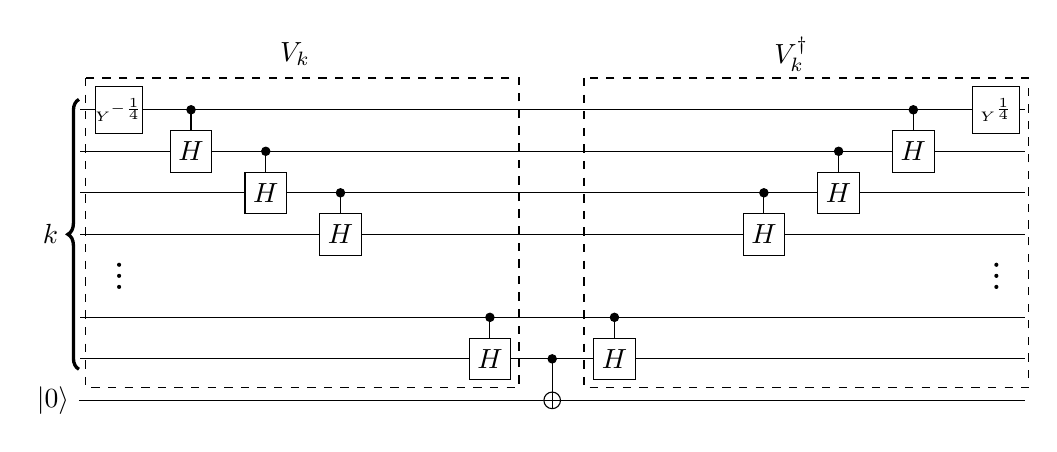
\begin{tikzpicture}[scale=1.000000,x=1pt,y=1pt]
\filldraw[color=white] (0.000000, -7.500000) rectangle (342.000000, 112.500000);
% Drawing wires
% Line 2: 1 W
\draw[color=black] (0.000000,105.000000) -- (342.000000,105.000000);
%   Deferring wire label at (0.000000,105.000000)
% Line 3: 2 W
\draw[color=black] (0.000000,90.000000) -- (342.000000,90.000000);
% Line 4: 3 W
\draw[color=black] (0.000000,75.000000) -- (342.000000,75.000000);
% Line 5: 4 W
\draw[color=black] (0.000000,60.000000) -- (342.000000,60.000000);
% Line 6: b W color=white
\draw[color=white] (0.000000,45.000000) -- (342.000000,45.000000);
% Line 7: m W
\draw[color=black] (0.000000,30.000000) -- (342.000000,30.000000);
% Line 8: n W
\draw[color=black] (0.000000,15.000000) -- (342.000000,15.000000);
\filldraw[color=white,fill=white] (0.000000,11.250000) rectangle (-4.000000,108.750000);
\draw[decorate,decoration={brace,amplitude = 4.000000pt},very thick] (0.000000,11.250000) -- (0.000000,108.750000);
\draw[color=black] (-4.000000,60.000000) node[left] {$k$};
% Line 10: 0 W \ket{0}
\draw[color=black] (0.000000,0.000000) -- (342.000000,0.000000);
\draw[color=black] (0.000000,0.000000) node[left] {$\ket{0}$};
% Done with wires; drawing the dots to represent continuity
%Left side
\fill (14.500000,41.000000) circle (0.75pt);
\fill (14.500000,45.000000) circle (0.75pt);
\fill (14.500000,49.000000) circle (0.75pt);
%Right side
\fill (331.50000,41.000000) circle (0.75pt);
\fill (331.50000,45.000000) circle (0.75pt);
\fill (331.50000,49.000000) circle (0.75pt);
%Drawing gates
% Line 12: 1 G:size=17 {\tiny $Y^{-1/4}$}
\begin{scope}
\draw[fill=white] (14.500000, 105.000000) +(-45.000000:12.020815pt and 12.020815pt) -- +(45.000000:12.020815pt and 12.020815pt) -- +(135.000000:12.020815pt and 12.020815pt) -- +(225.000000:12.020815pt and 12.020815pt) -- cycle;
\clip (14.500000, 105.000000) +(-45.000000:12.020815pt and 12.020815pt) -- +(45.000000:12.020815pt and 12.020815pt) -- +(135.000000:12.020815pt and 12.020815pt) -- +(225.000000:12.020815pt and 12.020815pt) -- cycle;
\draw (14.500000, 105.000000) node {{\tiny $Y^{-\frac{1}{4}}$}};
\end{scope}
% Line 13: 2 H:size=15 1
\draw (40.500000,105.000000) -- (40.500000,90.000000);
\begin{scope}
\draw[fill=white] (40.500000, 90.000000) +(-45.000000:10.606602pt and 10.606602pt) -- +(45.000000:10.606602pt and 10.606602pt) -- +(135.000000:10.606602pt and 10.606602pt) -- +(225.000000:10.606602pt and 10.606602pt) -- cycle;
\clip (40.500000, 90.000000) +(-45.000000:10.606602pt and 10.606602pt) -- +(45.000000:10.606602pt and 10.606602pt) -- +(135.000000:10.606602pt and 10.606602pt) -- +(225.000000:10.606602pt and 10.606602pt) -- cycle;
\draw (40.500000, 90.000000) node {$H$};
\end{scope}
\filldraw (40.500000, 105.000000) circle(1.500000pt);
% Line 14: 3 H:size=15 2
\draw (67.500000,90.000000) -- (67.500000,75.000000);
\begin{scope}
\draw[fill=white] (67.500000, 75.000000) +(-45.000000:10.606602pt and 10.606602pt) -- +(45.000000:10.606602pt and 10.606602pt) -- +(135.000000:10.606602pt and 10.606602pt) -- +(225.000000:10.606602pt and 10.606602pt) -- cycle;
\clip (67.500000, 75.000000) +(-45.000000:10.606602pt and 10.606602pt) -- +(45.000000:10.606602pt and 10.606602pt) -- +(135.000000:10.606602pt and 10.606602pt) -- +(225.000000:10.606602pt and 10.606602pt) -- cycle;
\draw (67.500000, 75.000000) node {$H$};
\end{scope}
\filldraw (67.500000, 90.000000) circle(1.500000pt);
% Line 15: 4 H:size=15 3
\draw (94.500000,75.000000) -- (94.500000,60.000000);
\begin{scope}
\draw[fill=white] (94.500000, 60.000000) +(-45.000000:10.606602pt and 10.606602pt) -- +(45.000000:10.606602pt and 10.606602pt) -- +(135.000000:10.606602pt and 10.606602pt) -- +(225.000000:10.606602pt and 10.606602pt) -- cycle;
\clip (94.500000, 60.000000) +(-45.000000:10.606602pt and 10.606602pt) -- +(45.000000:10.606602pt and 10.606602pt) -- +(135.000000:10.606602pt and 10.606602pt) -- +(225.000000:10.606602pt and 10.606602pt) -- cycle;
\draw (94.500000, 60.000000) node {$H$};
\end{scope}
\filldraw (94.500000, 75.000000) circle(1.500000pt);
% Line 16: b TOUCH
% Line 17: b G:size=15  \rotatebox{90}{...} color=white
\begin{scope}[color=white]
\begin{scope}[color=white]
\begin{scope}
\draw[fill=white] (121.500000, 45.000000) +(-45.000000:10.606602pt and 10.606602pt) -- +(45.000000:10.606602pt and 10.606602pt) -- +(135.000000:10.606602pt and 10.606602pt) -- +(225.000000:10.606602pt and 10.606602pt) -- cycle;
\clip (121.500000, 45.000000) +(-45.000000:10.606602pt and 10.606602pt) -- +(45.000000:10.606602pt and 10.606602pt) -- +(135.000000:10.606602pt and 10.606602pt) -- +(225.000000:10.606602pt and 10.606602pt) -- cycle;
\draw (121.500000, 45.000000) node {\rotatebox{90}{...}};
\end{scope}
\end{scope}
\end{scope}
% Line 18: n TOUCH
% Line 19: n H:size=15 m
\draw (148.500000,30.000000) -- (148.500000,15.000000);
\begin{scope}
\draw[fill=white] (148.500000, 15.000000) +(-45.000000:10.606602pt and 10.606602pt) -- +(45.000000:10.606602pt and 10.606602pt) -- +(135.000000:10.606602pt and 10.606602pt) -- +(225.000000:10.606602pt and 10.606602pt) -- cycle;
\clip (148.500000, 15.000000) +(-45.000000:10.606602pt and 10.606602pt) -- +(45.000000:10.606602pt and 10.606602pt) -- +(135.000000:10.606602pt and 10.606602pt) -- +(225.000000:10.606602pt and 10.606602pt) -- cycle;
\draw (148.500000, 15.000000) node {$H$};
\end{scope}
\filldraw (148.500000, 30.000000) circle(1.500000pt);
% Line 21: 0 C n
\draw (171.000000,15.000000) -- (171.000000,0.000000);
\begin{scope}
\draw[fill=white] (171.000000, 0.000000) circle(3.000000pt);
\clip (171.000000, 0.000000) circle(3.000000pt);
\draw (168.000000, 0.000000) -- (174.000000, 0.000000);
\draw (171.000000, -3.000000) -- (171.000000, 3.000000);
\end{scope}
\filldraw (171.000000, 15.000000) circle(1.500000pt);
% Line 22: n H:size=15 m
\draw (193.500000,30.000000) -- (193.500000,15.000000);
\begin{scope}
\draw[fill=white] (193.500000, 15.000000) +(-45.000000:10.606602pt and 10.606602pt) -- +(45.000000:10.606602pt and 10.606602pt) -- +(135.000000:10.606602pt and 10.606602pt) -- +(225.000000:10.606602pt and 10.606602pt) -- cycle;
\clip (193.500000, 15.000000) +(-45.000000:10.606602pt and 10.606602pt) -- +(45.000000:10.606602pt and 10.606602pt) -- +(135.000000:10.606602pt and 10.606602pt) -- +(225.000000:10.606602pt and 10.606602pt) -- cycle;
\draw (193.500000, 15.000000) node {$H$};
\end{scope}
\filldraw (193.500000, 30.000000) circle(1.500000pt);
% Line 23: b TOUCH
% Line 24: b G:size=15 \rotatebox{90}{...} color=white
\begin{scope}[color=white]
\begin{scope}[color=white]
\begin{scope}
\draw[fill=white] (220.500000, 45.000000) +(-45.000000:10.606602pt and 10.606602pt) -- +(45.000000:10.606602pt and 10.606602pt) -- +(135.000000:10.606602pt and 10.606602pt) -- +(225.000000:10.606602pt and 10.606602pt) -- cycle;
\clip (220.500000, 45.000000) +(-45.000000:10.606602pt and 10.606602pt) -- +(45.000000:10.606602pt and 10.606602pt) -- +(135.000000:10.606602pt and 10.606602pt) -- +(225.000000:10.606602pt and 10.606602pt) -- cycle;
\draw (220.500000, 45.000000) node {\rotatebox{90}{...}};
\end{scope}
\end{scope}
\end{scope}
% Line 25: 4 TOUCH
% Line 26: 4 H:size=15 3
\draw (247.500000,75.000000) -- (247.500000,60.000000);
\begin{scope}
\draw[fill=white] (247.500000, 60.000000) +(-45.000000:10.606602pt and 10.606602pt) -- +(45.000000:10.606602pt and 10.606602pt) -- +(135.000000:10.606602pt and 10.606602pt) -- +(225.000000:10.606602pt and 10.606602pt) -- cycle;
\clip (247.500000, 60.000000) +(-45.000000:10.606602pt and 10.606602pt) -- +(45.000000:10.606602pt and 10.606602pt) -- +(135.000000:10.606602pt and 10.606602pt) -- +(225.000000:10.606602pt and 10.606602pt) -- cycle;
\draw (247.500000, 60.000000) node {$H$};
\end{scope}
\filldraw (247.500000, 75.000000) circle(1.500000pt);
% Line 27: 3 H:size=15 2
\draw (274.500000,90.000000) -- (274.500000,75.000000);
\begin{scope}
\draw[fill=white] (274.500000, 75.000000) +(-45.000000:10.606602pt and 10.606602pt) -- +(45.000000:10.606602pt and 10.606602pt) -- +(135.000000:10.606602pt and 10.606602pt) -- +(225.000000:10.606602pt and 10.606602pt) -- cycle;
\clip (274.500000, 75.000000) +(-45.000000:10.606602pt and 10.606602pt) -- +(45.000000:10.606602pt and 10.606602pt) -- +(135.000000:10.606602pt and 10.606602pt) -- +(225.000000:10.606602pt and 10.606602pt) -- cycle;
\draw (274.500000, 75.000000) node {$H$};
\end{scope}
\filldraw (274.500000, 90.000000) circle(1.500000pt);
% Line 28: 2 H:size=15 1
\draw (301.500000,105.000000) -- (301.500000,90.000000);
\begin{scope}
\draw[fill=white] (301.500000, 90.000000) +(-45.000000:10.606602pt and 10.606602pt) -- +(45.000000:10.606602pt and 10.606602pt) -- +(135.000000:10.606602pt and 10.606602pt) -- +(225.000000:10.606602pt and 10.606602pt) -- cycle;
\clip (301.500000, 90.000000) +(-45.000000:10.606602pt and 10.606602pt) -- +(45.000000:10.606602pt and 10.606602pt) -- +(135.000000:10.606602pt and 10.606602pt) -- +(225.000000:10.606602pt and 10.606602pt) -- cycle;
\draw (301.500000, 90.000000) node {$H$};
\end{scope}
\filldraw (301.500000, 105.000000) circle(1.500000pt);
% Line 29: 1 G:size=17 {\tiny $Y^{1/4}$}
\begin{scope}
\draw[fill=white] (331.500000, 105.000000) +(-45.000000:12.020815pt and 12.020815pt) -- +(45.000000:12.020815pt and 12.020815pt) -- +(135.000000:12.020815pt and 12.020815pt) -- +(225.000000:12.020815pt and 12.020815pt) -- cycle;
\clip (331.500000, 105.000000) +(-45.000000:12.020815pt and 12.020815pt) -- +(45.000000:12.020815pt and 12.020815pt) -- +(135.000000:12.020815pt and 12.020815pt) -- +(225.000000:12.020815pt and 12.020815pt) -- cycle;
\draw (331.500000, 105.000000) node {{\tiny $Y^\frac{1}{4}$}};
\end{scope}
% Done with gates; drawing ending labels
% Done with ending labels; drawing cut lines and comments
% Line 20: 1 n @ 0 5 color=black style=dashed
\draw[draw opacity=1.000000,fill opacity=0.200000,color=black,dashed] (2.500000,116.500000) rectangle (159.000000,4.500000);
% Line 30: 1 n @ 7 12 color=black style=dashed
\draw[draw opacity=1.000000,fill opacity=0.200000,color=black,dashed] (182.500000,116.500000) rectangle (343.000000,4.500000);
%Labelling V_k left and right
\draw[color=black] (87.000000,125.000000) node[left] {$V_k$};
\draw[color=black] (267.000000,125.000000) node[left] {$V_k^\dagger$};
% Done with comments
\end{tikzpicture}
\caption{The circuit $U_k=V_k^\dagger CNOT_{(k,A)} V_k$.}
    \label{fig:CircuitUk}
\end{figure}

Our goal here is to prove that the circuit from Figure \ref{fig:CircuitUk} extracts the value $x_k$ while leaving the state mostly unperturbed. That is, we will prove the following lemma.

\begin{lemma}
Let $\textbf{x}=(x_1,\dots,x_k)\in\{0,1\}^k$ be a $k$ bit string, and $\ket{\textbf{x}_{enc}}$ its encoding.
\begin{equation}
|\bra{\textbf{x}_{enc}}\bra{x_k}U_k\ket{\textbf{x}_{enc}}\ket{0}|= \sqrt{1-\frac{\sin^2\frac{\pi}{8}}{2^{k-1}}}
\end{equation}
\label{lem:bit_extract}
\end{lemma}
\begin{proof}
We begin by noticing that we can split $U_k$ into $V_k^\dagger CNOT_{(k,A)}V_k$, where $V_k$ are unitaries that only act on the block of $k$ qubits and the controlled not operation acts on the last qubit of the block and the ancilla. The crucial part of the proof will be to understand the structure of  $V_k\ket{Enc(\vec{x})}$. Indeed, allow us to write  $V_k\ket{Enc(\vec{x})}$ as
\[V_k\ket{\textbf{x}_{enc}}=\ket{\psi}\ket{x_k}+\ket{\phi}\ket{\bar{x_k}},\]
For some vectors $\ket{\psi}$ and $\ket{\phi}$. Observe that the $CNOT$ with a target initialized at $\ket{0}$ simply copies into the ancillary register the value of the $k$-th bit of $V_k\ket{\textbf{x}_{enc}}$, hence we have
\begin{equation}
CNOT_{(k,A)}V_k\ket{\textbf{x}_{enc}}\ket{0}=\ket{\psi}\ket{x_k}\ket{x_k}+\ket{\phi}\ket{\bar{x_k}}\ket{\bar{x_k}}.
\end{equation}

Hence, the inner product that we are interested in reads
\begin{eqnarray}
|\bra{\textbf{x}_{enc}}\bra{x_k}V_k^\dagger CNOT_{(k,A)}V_k\ket{\textbf{x}_{enc}}\ket{0}|&=&|\left[\left(\bra{\psi}\bra{x_k}+\bra{\phi}\bra{\bar{x_k}}\right)\bra{x_k}\right]\left[\ket{\psi}\ket{x_k}\ket{x_k}+\ket{\phi}\ket{\bar{x_k}}\ket{\bar{x_k}}\right]|\\
&=&|\braket{\psi}{\psi}|=\sqrt{1-|\braket{\phi}{\phi}|^2}.
\end{eqnarray}

Now, we shall characterize $V_k\ket{\textbf{x}_{enc}}$ and prove that $|\ket{\phi}|$ is really small.

We begin by observing that the action of $Y^{\frac{1}{4}}$ on $\ket{\textbf{x}_{enc}}$ only afects the first qubit, mapping it to

\[Y^\frac{1}{4}\ket{x_1}_{x_{0}}=(-1)^{x_0}\cos\frac{\pi}{8}\ket{x_1}+(-1)^{1-x_0}\sin\frac{\pi}{8}\ket{1-x_1}.\]
This last equality can be deduced directly from Figure \ref{fig:bases} because rotating $\ket{0}, \ket{1}, \ket{+},$ and $\ket{-}$ by an angle $\frac{\pi}{8}$ on the block sphere is conceptually nothing more than writing these states in the basis $\{\ket{\xi_0}, \ket{\xi_1}\}$ and rename those states as $\ket{0}$ and $\ket{1}$. Hence, we can think of this rotation as splitting $\ket{\textbf{x}_{enc}}$ into two parts, one with $\ket{x_1}$ in the first register, and one with $\ket{1-x_1}$ in the same register.

\begin{figure}[t]
\centering
\begin{tikzpicture}
\draw[black, thick,->] (0,0) -- (0,3) node[above] {$\ket{1}$};
\draw[black, thick,->] (0,0) --(3,0) node[right] {$\ket{0}$};
\draw[black, dashed,->] (0,0) --(2.1213,2.1213) node[above] {$\ket{+}$};
\draw[black, dashed,->] (0,0) --(-2.1213,2.1213) node[above] {$\ket{-}$};
\draw[black, dotted,->] (0,0) --(2.7716,1.14805) node[right] {$\ket{\xi_0}$};
\draw[black, dotted,->] (0,0) --(-1.14805,2.7716) node[above] {$\ket{\xi_1}$};
\end{tikzpicture}
\caption{The basis $\{\ket{\xi_0}, \ket{\xi_1}\}$.}
\label{fig:bases}
\end{figure}

When one applies the second layer of the circuit $V_k$ on part of the state $Y^{\frac{1}{4}}\ket{\textbf{x}_{enc}}$ labeled by $x_1$ in the first register, one obtains 
\[\cos\frac{\pi}{8}(-1)^{x_0}CH_{1,2}\ket{x_1}\bigotimes_{j=2}^k\ket{x_j}_{x_{j-1}}=\cos\frac{\pi}{8}(-1)^{x_0}\ket{x_1}H^{2 x_1}\ket{x_2}\bigotimes_{j=3}^k\ket{x_j}_{x_{j-1}}\]
In fact, it follows by inspection that the entire circuit $V_k$ acting on this state will simply decode the rest of the bits. More interesting is the action of that first controlled Hadamard on the other branch, $\sin\frac{\pi}{8}(-1)^{1-x_0}\ket{1-x_1}\bigotimes_{j=2}^k\ket{x_j}_{x_{j-1}}$. In this branch we have

\begin{eqnarray}
&CH(1,2)\ket{1-x_1}\ket{x_{2(x_1)}}\bigotimes_{j=3}^k\ket{x_j}_{x_{j-1}}\\
&=\ket{1-x_1}H^{(1-x_1)}H^{x_1}\ket{x_2}\bigotimes_{j=3}^k\ket{x_j}_{x_{j-1}}\\
&=\ket{1-x_1}\left(\frac{\ket{1-x_2}+(-1)^{x_2}\ket{x_2}}{\sqrt2}\right)\bigotimes_{j=3}^k\ket{x_j}_{x_{j-1}}
\end{eqnarray}

In general, for any given $l<k$, every time the controll qubit is in the wrong state, the controlled Hadamard will split the target into a ket with $\ket{x_l}$ and one with $\ket{1-x_l}$. Then again, the next controlled Hadamard will decode the next bit correctly on the first branch, and, in fact, the remainder of the circuit will correctly decode the rest of the qubits.Meanwile, on the wrong branch, the next gate will split the next qubit into an equal superposition of the correct and incorrect bit values, and the same argument will apply. It is a simple exercise that the state at the end of the circuit will be
\begin{equation}
V_k\ket{\textbf{x}_{enc}}=\cos\frac{\pi}{8}\bigotimes_{i=1}^k\ket{x_i}+\sin\frac{\pi}{8}\sum_{l=1}^k\frac{1}{2^{\frac{l-1}{2}}}\left(\bigotimes_{i=1}^l\ket{1-x_i}\bigotimes_{j=l+1}^k\ket{x_j}\right)
\end{equation}
Finally, notice how this state can be written as
\[V_k\ket{\textbf{x}_{enc}}=\ket{\psi}\ket{x_k}+\ket{\phi}\ket{1-x_k},\quad \text{where} \quad \ket{\phi}=\sin\frac{\pi}{8}\frac{1}{2^{\frac{k-1}{2}}}\bigotimes_{i=1}^{k-1}\ket{1-x_i}\]

\end{proof}

%! \usetikzlibrary{decorations.pathreplacing,decorations.pathmorphing}
\begin{figure}
    \centering
    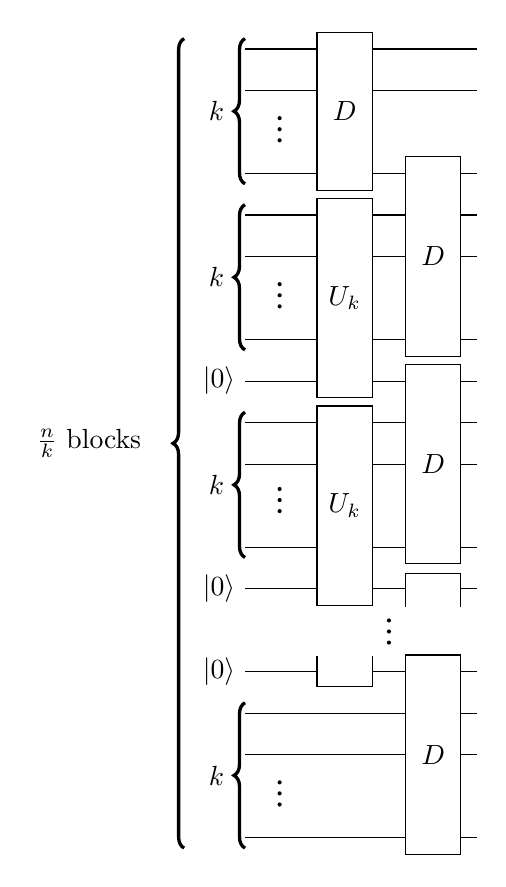
\begin{tikzpicture}[scale=1.000000,x=1pt,y=1pt]
\filldraw[color=white] (0.000000, -7.500000) rectangle (64.000000, 292.500000);
% Drawing wires
% Line 2: 1 W
\draw[color=black] (-20.000000,285.000000) -- (64.000000,285.000000);
%   Deferring wire label at (0.000000,285.000000)
% Line 3: 2 W
\draw[color=black] (-20.000000,270.000000) -- (64.000000,270.000000);
% Line 4: a W color=white
\draw[color=white] (-20.000000,255.000000) -- (64.000000,255.000000);
% Line 5: 4 W
\draw[color=black] (-20.000000,240.000000) -- (64.000000,240.000000);
%\filldraw[color=white,fill=white] (0.000000,236.250000) rectangle (-4.000000,288.750000);
\draw[decorate,decoration={brace,amplitude = 4.000000pt},very thick] (-20.000000,236.250000) -- (-20.000000,288.750000);
\draw[color=black] (-24.000000,262.500000) node[left] {$k$};
% Line 7: 5 W
\draw[color=black] (-20.000000,225.000000) -- (64.000000,225.000000);
%   Deferring wire label at (0.000000,225.000000)
% Line 8: 6 W
\draw[color=black] (-20.000000,210.000000) -- (64.000000,210.000000);
% Line 9: b W color=white
\draw[color=white] (-20.000000,195.000000) -- (64.000000,195.000000);
% Line 10: 7 W
\draw[color=black] (-20.000000,180.000000) -- (64.000000,180.000000);
%\filldraw[color=white,fill=white] (0.000000,176.250000) rectangle (-4.000000,228.750000);
\draw[decorate,decoration={brace,amplitude = 4.000000pt},very thick] (-20.000000,176.250000) -- (-20.000000,228.750000);
\draw[color=black] (-24.000000,202.500000) node[left] {$k$};
% Line 11: u W \ket{0}
\draw[color=black] (-20.000000,165.000000) -- (64.000000,165.000000);
\draw[color=black] (-20.000000,165.000000) node[left] {$\ket{0}$};
% Line 13: 8 W
\draw[color=black] (-20.000000,150.000000) -- (64.000000,150.000000);
%   Deferring wire label at (0.000000,150.000000)
% Line 14: 9 W
\draw[color=black] (-20.000000,135.000000) -- (64.000000,135.000000);
% Line 15: c W color=white
\draw[color=white] (-20.000000,120.000000) -- (64.000000,120.000000);
% Line 16: 10 W
\draw[color=black] (-20.000000,105.000000) -- (64.000000,105.000000);
%\filldraw[color=white,fill=white] (0.000000,101.250000) rectangle (-24.000000,153.750000);
\draw[decorate,decoration={brace,amplitude = 4.000000pt},very thick] (-20.000000,101.250000) -- (-20.000000,153.750000);
\draw[color=black] (-24.000000,127.500000) node[left] {$k$};
% Line 17: v W \ket{0}
\draw[color=black] (-20.000000,90.000000) -- (64.000000,90.000000);
\draw[color=black] (-20.000000,90.000000) node[left] {$\ket{0}$};
% Line 19: s W color=white
\draw[color=white] (-20.000000,75.000000) -- (64.000000,75.000000);
% Line 21: x W \ket{0}
\draw[color=black] (-20.000000,60.000000) -- (64.000000,60.000000);
\draw[color=black] (-20.000000,60.000000) node[left] {$\ket{0}$};
% Line 23: p W
\draw[color=black] (-20.000000,45.000000) -- (64.000000,45.000000);
%   Deferring wire label at (0.000000,45.000000)
% Line 24: q W
\draw[color=black] (-20.000000,30.000000) -- (64.000000,30.000000);
% Line 25: r W color=white
\draw[color=white] (-20.000000,15.000000) -- (64.000000,15.000000);
% Line 26: n W
\draw[color=black] (-20.000000,0.000000) -- (64.000000,0.000000);
%\filldraw[color=white,fill=white] (0.000000,-3.750000) rectangle (-4.000000,48.750000);
\draw[decorate,decoration={brace,amplitude = 4.000000pt},very thick] (-20.000000,-3.750000) -- (-20.000000,48.750000);
\draw[color=black] (-24.000000,22.500000) node[left] {$k$};
% Done with wires
%Big braces
\draw[decorate,decoration={brace,amplitude = 4.000000pt},very thick] (-42.000000,-3.750000) -- (-42.000000,288.750000);
\draw[color=black] (-54.000000,142.500000) node[left] {$\frac{n}{k} \text{ blocks}$};
%Drawing dots to represent continuity of the wires
\fill (-7.500000,252.000000) circle (0.75pt);
\fill (-7.500000,256.000000) circle (0.75pt);
\fill (-7.500000,260.000000) circle (0.75pt);

\fill (-7.500000,192.000000) circle (0.75pt);
\fill (-7.500000,196.000000) circle (0.75pt);
\fill (-7.500000,200.000000) circle (0.75pt);

\fill (-7.500000,118.000000) circle (0.75pt);
\fill (-7.500000,122.000000) circle (0.75pt);
\fill (-7.500000,126.000000) circle (0.75pt);

\fill (-7.500000,12.000000) circle (0.75pt);
\fill (-7.500000,16.000000) circle (0.75pt);
\fill (-7.500000,20.000000) circle (0.75pt);
%drawing gates
% Line 33: 1 2 a 4 G:size=20 $D$
\draw (16.000000,285.000000) -- (16.000000,240.000000);
\begin{scope}
\draw[fill=white] (16.000000, 262.500000) +(-45.000000:14.142136pt and 40.305087pt) -- +(45.000000:14.142136pt and 40.305087pt) -- +(135.000000:14.142136pt and 40.305087pt) -- +(225.000000:14.142136pt and 40.305087pt) -- cycle;
\clip (16.000000, 262.500000) +(-45.000000:14.142136pt and 40.305087pt) -- +(45.000000:14.142136pt and 40.305087pt) -- +(135.000000:14.142136pt and 40.305087pt) -- +(225.000000:14.142136pt and 40.305087pt) -- cycle;
\draw (16.000000, 262.500000) node {$D$};
\end{scope}
% Line 34: 5 6 b 7 u G:size=20 $U_k$
\draw (16.000000,225.000000) -- (16.000000,165.000000);
\begin{scope}
\draw[fill=white] (16.000000, 195.000000) +(-45.000000:14.142136pt and 50.911688pt) -- +(45.000000:14.142136pt and 50.911688pt) -- +(135.000000:14.142136pt and 50.911688pt) -- +(225.000000:14.142136pt and 50.911688pt) -- cycle;
\clip (16.000000, 195.000000) +(-45.000000:14.142136pt and 50.911688pt) -- +(45.000000:14.142136pt and 50.911688pt) -- +(135.000000:14.142136pt and 50.911688pt) -- +(225.000000:14.142136pt and 50.911688pt) -- cycle;
\draw (16.000000, 195.000000) node {$U_k$};
\end{scope}
% Line 35: 8 9 c 10 v G:size=20 $U_k$
\draw (16.000000,150.000000) -- (16.000000,90.000000);
\begin{scope}
\draw[fill=white] (16.000000, 120.000000) +(-45.000000:14.142136pt and 50.911688pt) -- +(45.000000:14.142136pt and 50.911688pt) -- +(135.000000:14.142136pt and 50.911688pt) -- +(225.000000:14.142136pt and 50.911688pt) -- cycle;
\clip (16.000000, 120.000000) +(-45.000000:14.142136pt and 50.911688pt) -- +(45.000000:14.142136pt and 50.911688pt) -- +(135.000000:14.142136pt and 50.911688pt) -- +(225.000000:14.142136pt and 50.911688pt) -- cycle;
\draw (16.000000, 120.000000) node {$U_k$};
\end{scope}
% Line 36: x TOUCH
% Line 38: 4 5 6 b 7 G:size=20 $D$
\draw (48.000000,240.000000) -- (48.000000,180.000000);
\begin{scope}
\draw[fill=white] (48.000000, 210.000000) +(-45.000000:14.142136pt and 50.911688pt) -- +(45.000000:14.142136pt and 50.911688pt) -- +(135.000000:14.142136pt and 50.911688pt) -- +(225.000000:14.142136pt and 50.911688pt) -- cycle;
\clip (48.000000, 210.000000) +(-45.000000:14.142136pt and 50.911688pt) -- +(45.000000:14.142136pt and 50.911688pt) -- +(135.000000:14.142136pt and 50.911688pt) -- +(225.000000:14.142136pt and 50.911688pt) -- cycle;
\draw (48.000000, 210.000000) node {$D$};
\end{scope}
% Line 39: u 8 9 c 10 G:size=20 $D$
\draw (48.000000,165.000000) -- (48.000000,105.000000);
\begin{scope}
\draw[fill=white] (48.000000, 135.000000) +(-45.000000:14.142136pt and 50.911688pt) -- +(45.000000:14.142136pt and 50.911688pt) -- +(135.000000:14.142136pt and 50.911688pt) -- +(225.000000:14.142136pt and 50.911688pt) -- cycle;
\clip (48.000000, 135.000000) +(-45.000000:14.142136pt and 50.911688pt) -- +(45.000000:14.142136pt and 50.911688pt) -- +(135.000000:14.142136pt and 50.911688pt) -- +(225.000000:14.142136pt and 50.911688pt) -- cycle;
\draw (48.000000, 135.000000) node {$D$};
\end{scope}
%Drawing part of the decoder D
\draw[fill=white, color=white] (38.000000,83.500000) rectangle (58.000000,95.500000);
\draw (38.000000,83.500000) -- (38.000000,95.500000);
\draw (58.000000,83.500000) -- (58.000000,95.500000);
\draw (38.000000,95.500000) -- (58.000000,95.500000);
%Drawing part of U_k
\draw[fill=white, color=white] (6.000000,54.500000) rectangle (26.000000,65.500000);
\draw (6.000000,54.500000) -- (6.000000,65.500000);
\draw (26.000000,54.500000) -- (26.000000,65.500000);
\draw (6.000000,54.500000) -- (26.000000,54.500000);
%Drawing dots to represent continuity of the gates
\fill (32.000000,70.500000) circle (0.75pt);
\fill (32.000000,74.500000) circle (0.75pt);
\fill (32.000000,78.500000) circle (0.75pt);
% Line 40: x p q r n G:size=20 $D$
\draw (48.000000,60.000000) -- (48.000000,0.000000);
\begin{scope}
\draw[fill=white] (48.000000, 30.000000) +(-45.000000:14.142136pt and 50.911688pt) -- +(45.000000:14.142136pt and 50.911688pt) -- +(135.000000:14.142136pt and 50.911688pt) -- +(225.000000:14.142136pt and 50.911688pt) -- cycle;
\clip (48.000000, 30.000000) +(-45.000000:14.142136pt and 50.911688pt) -- +(45.000000:14.142136pt and 50.911688pt) -- +(135.000000:14.142136pt and 50.911688pt) -- +(225.000000:14.142136pt and 50.911688pt) -- cycle;
\draw (48.000000, 30.000000) node {$D$};
\end{scope}
% Done with gates; drawing ending labels
% Done with ending labels; drawing cut lines and comments
% Done with comments
\end{tikzpicture}
\hspace{2cm}
%The circuit for the gate D
\begin{tikzpicture}[scale=1.000000,x=1pt,y=1pt]
\filldraw[color=white] (0.000000, 98.500000) rectangle (155.000000, 137.500000);
% Drawing wires
% Line 2: 1 W
\draw[color=black] (-20.000000,180.000000) -- (155.000000,180.000000);
% Line 3: 2 W
\draw[color=black] (-20.000000,165.000000) -- (155.000000,165.000000);
% Line 4: 3 W
\draw[color=black] (-20.000000,150.000000) -- (155.000000,150.000000);
% Line 5: a W color=white
\draw[color=white] (-20.000000,135.000000) -- (155.000000,135.000000);
% Line 6: 4 W
\draw[color=black] (-20.000000,120.000000) -- (155.000000,120.000000);
% Line 7: 5 W
\draw[color=black] (-20.000000,105.000000) -- (155.000000,105.000000);
\draw[decorate,decoration={brace,amplitude = 4.000000pt},very thick] (-20.000000,101.250000) -- (-20.000000,183.750000);
\draw[color=black] (-24.000000,142.500000) node[left] {$t$};
% Done with wires
%Drawing dots to represent continuity of the wires
\fill (-8.000000,132.500000) circle (0.75pt);
\fill (-8.000000,136.500000) circle (0.75pt);
\fill (-8.000000,140.500000) circle (0.75pt);
%drawing gates
% Line 9: 1 2 3 a 4 5 G:size=20 $D$
\draw (16.000000,180.000000) -- (16.000000,105.000000);
\begin{scope}
\draw[fill=white] (16.000000, 142.500000) +(-45.000000:14.142136pt and 61.518290pt) -- +(45.000000:14.142136pt and 61.518290pt) -- +(135.000000:14.142136pt and 61.518290pt) -- +(225.000000:14.142136pt and 61.518290pt) -- cycle;
\clip (16.000000, 37.500000) +(-45.000000:14.142136pt and 61.518290pt) -- +(45.000000:14.142136pt and 61.518290pt) -- +(135.000000:14.142136pt and 61.518290pt) -- +(225.000000:14.142136pt and 61.518290pt) -- cycle;
\draw (16.000000, 142.500000) node {$D$};
\end{scope}
\draw (16.000000, 142.500000) node {$D$};
% Line 10: =
\draw[fill=white,color=white] (38.000000, 99.000000) rectangle (53.000000, 186.000000);
\draw (45.500000, 142.500000) node {$=$};
% Line 11: 2 H 1
\draw (71.000000,180.000000) -- (71.000000,165.000000);
\begin{scope}
\draw[fill=white] (71.000000, 165.000000) +(-45.000000:8.485281pt and 8.485281pt) -- +(45.000000:8.485281pt and 8.485281pt) -- +(135.000000:8.485281pt and 8.485281pt) -- +(225.000000:8.485281pt and 8.485281pt) -- cycle;
\clip (71.000000, 165.000000) +(-45.000000:8.485281pt and 8.485281pt) -- +(45.000000:8.485281pt and 8.485281pt) -- +(135.000000:8.485281pt and 8.485281pt) -- +(225.000000:8.485281pt and 8.485281pt) -- cycle;
\draw (71.000000, 165.000000) node {$H$};
\end{scope}
\filldraw (71.000000, 180.000000) circle(1.500000pt);
% Line 12: 3 H 2
\draw (95.000000,165.000000) -- (95.000000,150.000000);
\begin{scope}
\draw[fill=white] (95.000000, 150.000000) +(-45.000000:8.485281pt and 8.485281pt) -- +(45.000000:8.485281pt and 8.485281pt) -- +(135.000000:8.485281pt and 8.485281pt) -- +(225.000000:8.485281pt and 8.485281pt) -- cycle;
\clip (95.000000, 150.000000) +(-45.000000:8.485281pt and 8.485281pt) -- +(45.000000:8.485281pt and 8.485281pt) -- +(135.000000:8.485281pt and 8.485281pt) -- +(225.000000:8.485281pt and 8.485281pt) -- cycle;
\draw (95.000000, 150.000000) node {$H$};
\end{scope}
\filldraw (95.000000, 165.000000) circle(1.500000pt);
% Line 13: a TOUCH
% Line 14: a G $B$ color=white
\begin{scope}[color=white]
\begin{scope}[color=white]
\begin{scope}
\draw[fill=white] (119.000000, 135.000000) +(-45.000000:8.485281pt and 8.485281pt) -- +(45.000000:8.485281pt and 8.485281pt) -- +(135.000000:8.485281pt and 8.485281pt) -- +(225.000000:8.485281pt and 8.485281pt) -- cycle;
\clip (119.000000, 135.000000) +(-45.000000:8.485281pt and 8.485281pt) -- +(45.000000:8.485281pt and 8.485281pt) -- +(135.000000:8.485281pt and 8.485281pt) -- +(225.000000:8.485281pt and 8.485281pt) -- cycle;
\draw (119.000000, 135.000000) node {$B$};
\end{scope}
\end{scope}
\end{scope}
% Line 15: 4 TOUCH
% Line 16: 5 H 4
\draw (143.000000,120.000000) -- (143.000000,105.000000);
\begin{scope}
\draw[fill=white] (143.000000, 105.000000) +(-45.000000:8.485281pt and 8.485281pt) -- +(45.000000:8.485281pt and 8.485281pt) -- +(135.000000:8.485281pt and 8.485281pt) -- +(225.000000:8.485281pt and 8.485281pt) -- cycle;
\clip (143.000000, 105.000000) +(-45.000000:8.485281pt and 8.485281pt) -- +(45.000000:8.485281pt and 8.485281pt) -- +(135.000000:8.485281pt and 8.485281pt) -- +(225.000000:8.485281pt and 8.485281pt) -- cycle;
\draw (143.000000, 105.000000) node {$H$};
\end{scope}
\filldraw (143.000000, 120.000000) circle(1.500000pt);
%Drawing partial gate
%\filldraw (122.000000, 150.000000) circle(1.500000pt);
%\draw (122.00000, 150.0000) -- (122.0000, 145.0000);
% Done with gates
%Drawing dots to represent continuity of the H gates
\fill (122.000000,132.500000) circle (0.75pt);
\fill (122.000000,136.500000) circle (0.75pt);
\fill (122.000000,140.500000) circle (0.75pt);
\end{tikzpicture}
\caption{The circuit on the left is the entire decoding circuit. The circuit on the right is the honest decoder.}
\label{fig:FullDecoder}
\end{figure}


Let us think about what this lemma for a second. What we have proved is that this little circuit does not just extract the value $x_k$ encoded in the last qubit of $\ket{\textbf{x}_{enc}}$ with very high probability, it actually does so while barley disturbing the state in the first $k-1$ qubits of the block. The next step is now dividing our $n$-qubit encoded state into $n/k$ blocks of size $k$ and run the circuit of Figure \ref{fig:CircuitUk} parallelly in each block. Now, if we run the honest decoder in each block with the first Hadamard of the circuit controlled on the ancilla of the previous block, we would find that the state is decoded almost exactly since the state in these qubits is very near the original encoded state and the state of that ancilla is very near the comutational basis state encoding the right bit of information. Refer to Figure \ref{fig:FullDecoder} for the entire decoding circuit.\\

For any particular block $B_i$, Lemma \ref{lem:bit_extract} implies that the amplitude of the ancilla on the state $\ket{x_{i_k}}$ will be  bigger than $ \sqrt{1-\frac{\sin^2\frac{\pi}{8}}{2^{k-1}}}$. Call this ancillary qubit $A_i$. At the same time, if we apply the same lemma to the block $B_{i+1}$, we would get that the state in the qubits of the block would have an overlap with $\ket{\textbf{x}^{(i+1)}_{enc}}$ which is also bigger than $ \sqrt{1-\frac{\sin^2\frac{\pi}{8}}{2^{k-1}}}$.\\

All this implies that if we take the state on the ancilla $A_i$ and the qubits of the block $B_{i+1}$, we would have amplitude at least $ \sqrt{1-\frac{\sin^2\frac{\pi}{8}}{2^{k-1}}}^2$ on the state $\ket{x_{i_k}}\ket{\textbf{x}^{(i+1)}_{enc}}$.\\

By construction, applying the waterfall circuit to the latter state will result in perfect decoding of the bits of block $B_{i+1}$. Hence, applying the whaterfall circuit to the output of the first stage to the ancilla $A_i$ and the qubits of the block $B_{i+1}$ will result in a state with an overlap bigger or equal than $\sqrt{1-\frac{\sin^2\frac{\pi}{8}}{2^{k-1}}}^2$ with the state $\ket{x_{i_k}}\ket{\textbf{x}^{(i+1)}}$ . Finally, observe that we can apply this waterfall circuit with depth $k$ to every block. The amplitude of the  joint state of all $n/k$ blocks in the state $\ket{\textbf{x}}$ will then be bigger than
\begin{equation}
 \left(1-\frac{\sin^2\frac{\pi}{8}}{2^{k-1}}\right)^{n/k}.
\end{equation}

Accordingly, the probability of obtaining the right string $(x_1,\dots,x_n)$ upon measuring the output state in the computational basis will be the square of that. Choosing the depth of the blocks to be $k=q\log n$ will result in a success probability of decoding of at least

\begin{equation}
 \left(1-\frac{\sin^2\frac{\pi}{8}}{2^{k-1}}\right)^{2n/k}=1-O\left(\frac{1}{qn^{q-1}\log n}\right)
\end{equation}


\end{document}